

\begin{table}[H]
	\centering
	\begin{tabular}{|l|c|c|c|c|c|c|c|c|}
		\hline
		\multicolumn{1}{|c|}{\textbf{Solution}} & \multicolumn{1}{|c|}{RTL} & \multicolumn{1}{|c|}{Status} & \multicolumn{3}{c|}{\textbf{Latency}} & \multicolumn{3}{c|}{\textbf{Interval}} \\
		& &  & min & avg & max & min & avg & max \\
		\hline
		1 & VHDL & Pass & 58 & 58 & 58 & NA & NA & NA \\
		\hline
		2 & VHDL & Pass & 38 & 38 & 38 & NA & NA & NA \\
		\hline
		3 & VHDL & Pass & 58 & 58 & 58 & NA & NA & NA \\
		\hline
		4 & VHDL & Pass & 56 & 56 & 56 & NA & NA & NA \\
		\hline
		5 & VHDL & Pass & 37 & 37 & 37 & NA & NA & NA \\
		\hline
		6 &  &  &  &  &  &  &  &  \\
		\tabitem columnIndex, values, x & VHDL & Pass & 37 & 37 & 37 & NA & NA & NA \\
		\tabitem columnIndex & VHDL & Pass & 37 & 37 & 37 & NA & NA & NA \\
		\tabitem values & VHDL & Pass & 37 & 37 & 37 & NA & NA & NA \\
		\tabitem x & VHDL & Pass & 37 & 37 & 37 & NA & NA & NA \\
		\hline
		7 & VHDL & Pass & 38 & 38 & 38 & NA & NA & NA \\
		\hline
		8 &  &  &  &  &  &  &  &  \\
		\tabitem columnIndex, values, x & VHDL & Pass & 33 & 33 & 33 & NA & NA & NA \\
		\tabitem columnIndex & VHDL & Pass & 37 & 37 & 37 & NA & NA & NA \\
		\tabitem values & VHDL & Pass & 37 & 37 & 37 & NA & NA & NA \\
		\tabitem x & VHDL & Pass & 33 & 33 & 33 & NA & NA & NA \\
		\hline
		9 & VHDL & Pass & 34 & 34 & 34 & NA & NA & NA \\
		\hline
		10 &  &  &  &  &  &  &  &  \\
		\tabitem columnIndex, values, x & VHDL & Pass & 61 & 61 & 61 & NA & NA & NA \\
		\tabitem columnIndex & VHDL & Pass & 69 & 69 & 69 & NA & NA & NA \\
		\tabitem values & VHDL & Pass & 69 & 69 & 69 & NA & NA & NA \\
		\tabitem x & VHDL & Pass & 61 & 61 & 61 & NA & NA & NA \\
		\hline
		11 &  &  &  &  &  &  &  &  \\
		\tabitem columnIndex, values, x & VHDL & Pass & 64 & 64 & 64 & NA & NA & NA \\
		\tabitem columnIndex & VHDL & Pass & 72 & 72 & 72 & NA & NA & NA \\
		\tabitem values & VHDL & Pass & 72 & 72 & 72 & NA & NA & NA \\
		\tabitem x & VHDL & Pass & 64 & 64 & 64 & NA & NA & NA \\
		\hline
	\end{tabular}
	\caption{HLS Conclusions C/RTL Cosimulation Report }
	\label{tab:hls-conclusions-cosimulation-report}
\end{table}


\begin{figure}
	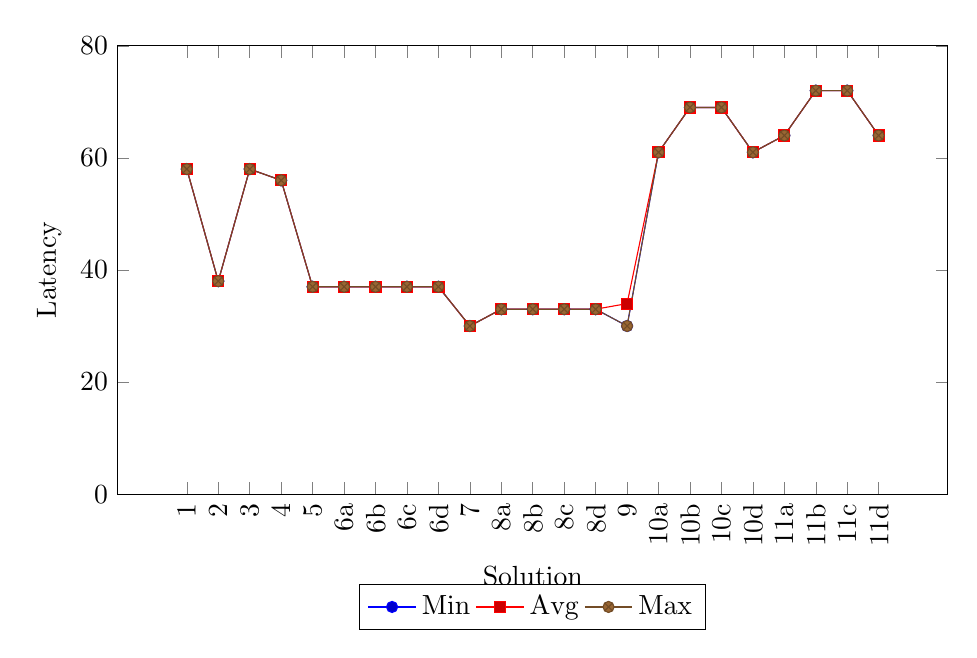
\begin{tikzpicture}
		\begin{axis}[
			symbolic x coords={1, 2, 3, 4, 5, 6a, 6b, 6c, 6d, 7, 8a, 8b, 8c, 8d, 9, 10a, 10b, 10c, 10d, 11a, 11b, 11c, 11d},
			xtick=data,
			ymin=0,
			ymax=80,
			ylabel={Latency},
			xlabel={Solution},
			legend style={at={(0.5,-0.20)}, anchor=north, legend columns=-1},
			width=1\textwidth,
			height=0.6\textwidth,
			xticklabel style={rotate=90, anchor=east},
			]
			\addplot coordinates {
				(1,58) (2,38) (3,58) (4,56) (5,37) (6a,37) (6b,37) (6c,37) (6d,37) (7,30) (8a,33) (8b,33) (8c,33) (8d,33) (9,30) (10a,61) (10b,69) (10c,69) (10d,61) (11a,64) (11b,72) (11c,72) (11d,64)
			};
			\addplot coordinates {
				(1,58) (2,38) (3,58) (4,56) (5,37) (6a,37) (6b,37) (6c,37) (6d,37) (7,30) (8a,33) (8b,33) (8c,33) (8d,33) (9,34) (10a,61) (10b,69) (10c,69) (10d,61) (11a,64) (11b,72) (11c,72) (11d,64)
			};
			\addplot coordinates {
				(1,58) (2,38) (3,58) (4,56) (5,37) (6a,37) (6b,37) (6c,37) (6d,37) (7,30) (8a,33) (8b,33) (8c,33) (8d,33) (9,30) (10a,61) (10b,69) (10c,69) (10d,61) (11a,64) (11b,72) (11c,72) (11d,64)
			};
			\legend{Min,Avg,Max}
		\end{axis}
	\end{tikzpicture}
	\caption{Latency measurements for different solutions}
	\label{fig:latency-measurements}
\end{figure}





\begin{table}[H]
	\centering
	\begin{tabular}{|l|c|c|c|c|c|c|c|c|}
		\hline
		\textbf{Solution} & \textbf{SLICE} & \textbf{LUT} & \textbf{FF} & \textbf{DSP} & \textbf{BRAM} & \textbf{CP} & \textbf{CP} & \textbf{CP} \\
		& & & & & & \textbf{required} & \textbf{achieved} & \textbf{achieved}\\
		& & & & & & & \textbf{post-} & \textbf{post-}\\
		& & & & & & & \textbf{synthesis} & \textbf{implementation}\\
		\hline
		1 & 48 & 93 & 161 & 3 & 0 & 10 & 5.745 & 5.692 \\
		\hline
		2 & 38 & 115 & 139 & 3 & 0 & 10 & 5.745 & 5.718 \\
		\hline
		3 & 48 & 94 & 161 & 3 & 0 & 10 & 5.745 & 5.692 \\
		\hline
		4 & 83 & 186 & 292 & 3 & 0 & 10 & 5.745 & 5.692 \\
		\hline
		5 & 69 & 184 & 196 & 6 & 0 & 10 & 7.927 & 7.465 \\
		\hline
		6 &  &  &  &  &  &  &  &  \\
		\tabitem columnIndex, values, x & 113 & 316 & 198 & 6 & 0 & 10 & 7.927 & 7.799 \\
		\tabitem columnIndex & 84 & 259 & 224 & 6 & 0 & 10 & 7.472 & 7.843 \\
		\tabitem values & 99 & 327 & 224 & 6 & 0 & 10 & 7.502 & 8.184 \\
		\tabitem x & 99 & 250 & 198 & 6 & 0 & 10 & 6.541 & 6.931 \\
		\hline
		7 & 75 & 248 & 131 & 3 & 0 & 10 & 5.745 & 6.120 \\
		\hline
		8 &  &  &  &  &  &  &  &  \\
		\tabitem columnIndex, values, x & 123 & 343 & 315 & 6 & 0 & 10 & 6.540 & 6.571 \\
		\tabitem columnIndex & 85 & 261 & 226 & 6 & 0 & 10 & 7.496 & 7.654 \\
		\tabitem values & 92 & 274 & 196 & 6 & 0 & 10 & 7.927 & 7.780 \\
		\tabitem x & 104 & 248 & 313 & 6 & 0 & 10 & 6.540 & 6.844 \\
		\hline
		9 & 75 & 248 & 131 & 3 & 0 & 10 & 5.745 & 6.120 \\
		\hline
		10 &  &  &  &  &  &  &  &  \\
		\tabitem columnIndex, values, x & 204 & 558 & 449 & 6 & 0 & 10 & 6.540 & 6.840 \\
		\tabitem columnIndex & 83 & 268 & 230 & 6 & 0 & 10 & 7.496 & 8.115 \\
		\tabitem values & 117 & 342 & 199 & 6 & 0 & 10 & 7.927 & 7.603 \\
		\tabitem x & 143 & 311 & 444 & 6 & 0 & 10 & 6.540 & 6.790 \\
		\hline
		11 &  &  &  &  &  &  &  &  \\
		\tabitem columnIndex, values, x & 179 & 454 & 450 & 6 & 0 & 10 & 6.541 & 6.677 \\
		\tabitem columnIndex & 90 & 267 & 227 & 6 & 0 & 10 & 7.489 & 7.664 \\
		\tabitem values & 122 & 391 & 232 & 6 & 0 & 10 & 7.506 & 7.768 \\
		\tabitem x & 143 & 311 & 444 & 6 & 0 & 10 & 6.540 & 6.790 \\
		\hline
	\end{tabular}
	\caption{HLS Conclusions Export RTL Report}
	\label{tab:hls-conclusions-export-rtl-report}
\end{table}




\begin{filecontents}{data.csv}
	Solution,SLICE,LUT,FF,DSP,BRAM,CP\_required,CP\_achieved\_post\_synthesis,CP\_achieved\_post\_implementation
	1,48,93,161,3,0,10,5.745,5.692
	2,38,115,139,3,0,10,5.745,5.718
	3,48,94,161,3,0,10,5.745,5.692
	4,83,186,292,3,0,10,5.745,5.692
	5,69,184,196,6,0,10,7.927,7.465
	6a,113,316,198,6,0,10,7.927,7.799
	6b,84,259,224,6,0,10,7.472,7.843
	6c,99,327,224,6,0,10,7.502,8.184
	6d,99,250,198,6,0,10,6.541,6.931
	7,75,248,131,3,0,10,5.745,6.120
	8a,123,343,315,6,0,10,6.540,6.571
	8b,85,261,226,6,0,10,7.496,7.654
	8c,92,274,196,6,0,10,7.927,7.780
	8d,104,248,313,6,0,10,6.540,6.844
	9,75,248,131,3,0,10,5.745,6.120
	10a,204,558,449,6,0,10,6.540,6.840
	10b,83,268,230,6,0,10,7.496,8.115
	10c,117,342,199,6,0,10,7.927,7.603
	10d,143,311,444,6,0,10,6.540,6.790
	11a,179,454,450,6,0,10,6.541,6.677
	11b,90,267,227,6,0,10,7.489,7.664
	11c,122,391,232,6,0,10,7.506,7.768
	11d,143,311,444,6,0,10,6.540,6.790
\end{filecontents}

	
\begin{figure}
	\centering
	\begin{tikzpicture}
		\begin{axis}[
			symbolic x coords={1, 2, 3, 4, 5, 6a, 6b, 6c, 6d, 7, 8a, 8b, 8c, 8d, 9, 10a, 10b, 10c, 10d, 11a, 11b, 11c, 11d},
			xtick=data,
			xlabel={Solution},
			ylabel={\#},
			xticklabel style={rotate=90, anchor=east},
			width=1\textwidth,
			height=0.6\textwidth,
			enlarge x limits=0.05,
			legend style={at={(0.5,-0.15)}, anchor=north,legend columns=-1}
			]
			\addplot table [x=Solution, y=SLICE, col sep=comma] {data.csv};
			\addplot table [x=Solution, y=LUT, col sep=comma] {data.csv};
			\addplot table [x=Solution, y=FF, col sep=comma] {data.csv};
			\addplot table [x=Solution, y=DSP, col sep=comma] {data.csv};
			\addplot table [x=Solution, y=BRAM, col sep=comma] {data.csv};
			\legend{SLICE, LUT, FF, DSP, BRAM}
		\end{axis}
	\end{tikzpicture}
	\caption{Utilization Export RTL Plot}
	\label{fig:utilization-export-rtl-plot}
\end{figure}


	